\section{Conclusion and Learnings} \label{section:luckypatcher-learnings}
\begin{itemize}
    \item result of patching, which applications work in which modes on unrooted devices
    \item since this can be tested it means they can also be sold on blackmarkets
    \item explenation of results, lvl (most time), amazon (always), samsung
    \item comprehension of luckypatcher
    \item instead of patching inital call, library itself is patched since it could call necessary code
    \item known bytecode patterns, replace with custom, prevent automatic patching
    \item in addition: does only attack library -> tampering checks?
    \item amazon, samsung cannot be fixed inside library, company has to act
    \item abstact presentation how attack works
    \item easy to attack since always this pattern if(someRights != null){
           // you have granted rights.
       } else {
           // You don't have any rights for the feature in cause. Try
           // some features. (Currently not supporting multiple 'features')
       } which can be attacked easily by voiding one result (see bytecode)
       \item the result is unary check
    \item since many applications are succesfully attacked with automatic mode, high motivation to modify library to be unique
\end{itemize}

\begin{figure}[h]
    \centering
    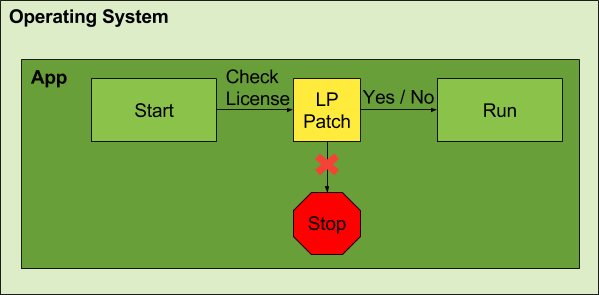
\includegraphics[width=0.8\textwidth]{data/verificationNowAttack.png}
    \caption{Abstraction of the current attack on the license verification mechanism}
    \label{fig:verificationNowAttack}
\end{figure}
